\documentclass[twocolumn,floatfix,aps,prd,superscriptaddress,nofootinbib]{revtex4-2}

% Engine guard: glyphtounicode and \pdfgentounicode are pdfTeX primitives.
% Under LuaLaTeX/XeLaTeX they are undefined and the run aborts in the preamble.
\usepackage{iftex}
\ifPDFTeX
  \usepackage[utf8]{inputenc}
  \usepackage[T1]{fontenc}
  \usepackage{lmodern}
  \input{glyphtounicode}
  \pdfgentounicode=1
\else
  \usepackage{fontspec}
  \setmainfont{Latin Modern Roman}
  \setsansfont{Latin Modern Sans}
  \setmonofont{Latin Modern Mono}
\fi
\usepackage{graphicx}
\usepackage{amssymb}
\usepackage{amsmath}
\usepackage{xcolor}
\usepackage{hyperref}
\usepackage{placeins}
\usepackage[protrusion=true,expansion=false]{microtype}
\usepackage{tikz}
\usetikzlibrary{positioning,arrows.meta}

% Half-page figure* strips must ride at the top of a text page, not own a
% float page of their own (the binary paper's Fig. 2 lesson).
\AtBeginDocument{%
  \renewcommand{\dbltopfraction}{0.92}%
  \renewcommand{\dblfloatpagefraction}{0.55}%
  \renewcommand{\textfraction}{0.1}%
  \setcounter{dbltopnumber}{2}%
}

\makeatletter
\newcommand{\packfloatpages}{%
  \setlength{\@fptop}{0pt}%
  \setlength{\@fpsep}{12pt}%
  \setlength{\@fpbot}{0pt plus 1fil}%
  \setlength{\@dblfptop}{0pt}%
  \setlength{\@dblfpsep}{12pt}%
  \setlength{\@dblfpbot}{0pt plus 1fil}%
}
\makeatother

\graphicspath{{figures/}{../../../results/optimisation/figures/}}

\hypersetup{
    colorlinks=true,
    linkcolor=blue,
    filecolor=magenta,
    urlcolor=blue,
    citecolor=blue,
}
\urlstyle{same}
\emergencystretch=2em

% Generated by claims/claims.py tex; edit the selection ledger, not this file.
\newcommand{\clmModelsRows}{%
\multicolumn{5}{l}{Drainhole, $150\times30$ search grid} \\
D0 & $1.199$ & $0.227$ & $0.485$ & $0.274$ \\
D21 & $1.171$ & $0.762$ & $0.351$ & $0.206$ \\
D30 & $0.740$ & $0.607$ & $0.201$ & $-0.664$ \\
D80 & $0.234$ & $0.083$ & $0.504$ & $1.187$ \\
D90 & $0.150$ & $-0.337$ & $0.366$ & $0.445$ \\
\hline
\multicolumn{5}{l}{Symmetric, $150\times30$ search grid} \\
S0 & $1.198$ & $2.433$ & $-0.046$ & $1.197$ \\
S27 & $0.855$ & $3.232$ & $3.776$ & $-0.256$ \\
S50 & $0.962$ & $3.739$ & $0.922$ & $-0.828$ \\
S85 & $0.425$ & $2.438$ & $4.267$ & $0.445$ \\
\hline
\multicolumn{5}{l}{Selected $210\times42$ solution} \\
D21$^\star$ & $1.023$ & $0.672$ & $0.048$ & $0.310$ \\
%
}
\newcommand{\clmExoticityRows}{%
\multicolumn{4}{l}{Drainhole, $150\times30$ search grid} \\
D0 & $1.839$ & $4.898$ & $-62.5\%$ \\
D21 & $1.785$ & $4.645$ & $-61.6\%$ \\
D30 & $1.880$ & $4.376$ & $-57.0\%$ \\
D80 & $1.105$ & $1.419$ & $-22.2\%$ \\
D90 & $0.787$ & $0.600$ & $+31.3\%$ \\
\hline
\multicolumn{4}{l}{Symmetric, $150\times30$ search grid} \\
S0 & $1.627$ & $3.142$ & $-48.2\%$ \\
S27 & $1.634$ & $2.994$ & $-45.4\%$ \\
S50 & $1.477$ & $2.625$ & $-43.7\%$ \\
S85 & $1.098$ & $1.462$ & $-24.9\%$ \\
\hline
\multicolumn{4}{l}{Selected $210\times42$ solution} \\
D21$^\star$ & $1.829$ & $4.645$ & $-60.6\%$ \\
%
}
\newcommand{\clmOrderRows}{%
Ham L0 & 2.67 / 2.77 & 1.09 / 3.13 & 4.66 / 4.35 & 4.39 / 4.27 & 4.28 / 4.30 \\
Mom L0 & 2.45 / 2.60 & 0.47 / 3.25 & 4.98 / 4.84 & 4.42 / 4.46 & 4.32 / 4.41 \\
Ham L1 & 2.12 / 2.38 & 2.80 / 2.49 & 3.95 / 2.46 & 2.33 / 2.47 & 2.15 / 2.39 \\
Mom L1 & 2.00 / 2.33 & 4.99 / 3.30 & 7.08 / 2.71 & 3.70 / 3.02 & 4.28 / 2.51 \\
Ham L2 & 2.17 / 2.43 & 2.21 / 2.49 & 2.35 / 2.50 & 3.45 / 3.12 & 3.78 / 3.90 \\
Mom L2 & 2.39 / 2.47 & 2.23 / 2.50 & 2.62 / 2.94 & 3.19 / 3.63 & 3.19 / 3.53 \\
Ham L3 & 4.03 / 4.18 & 4.10 / 4.21 & 4.14 / 4.23 & 4.20 / 4.24 & 4.33 / 4.25 \\
Mom L3 & 3.93 / 4.26 & 3.94 / 4.28 & 3.91 / 4.24 & 3.86 / 4.11 & 3.93 / 3.93 \\
%
}
\newcommand{\clmDsearchX}{%
1.785%
}
\newcommand{\clmDfineX}{%
1.829%
}
\newcommand{\clmDfineReduction}{%
60.6%
}
\newcommand{\clmDfineReductionRounded}{%
61%
}
\newcommand{\clmDfineEoneNine}{%
1.6\times10^{-10}%
}
\newcommand{\clmDfineEc}{%
4.3\times10^{-10}%
}
\newcommand{\clmContractionLow}{%
58.3%
}
\newcommand{\clmContractionMid}{%
67.3%
}
\newcommand{\clmContractionHigh}{%
80.7%
}
\newcommand{\clmGrowthClassicalTau}{%
6.59%
}
\newcommand{\clmGrowthPotentialTau}{%
9.49%
}
\newcommand{\clmGrowthReduction}{%
31%
}


\begin{document}

\raggedbottom

\title{Minimizing exotic matter in rotating Ellis--Bronnikov wormholes}

\author{Nikita M. Shirokov}
\email{shirokov.nm@phystech.edu}
\affiliation{\textit{Moscow Institute of Physics and Technology, Moscow, Russia}}
\author{Ilya Nachevsky}
\email{ommnammashivaya@gmail.com}
\affiliation{\textit{Higher School of Economics, Moscow, Russia}}
\date{\today}

\begin{abstract}
A confining scalar potential can reduce the exotic matter supporting a stationary rotating Ellis--Bronnikov wormhole. We search a four-parameter potential family at fixed equatorial throat radius and angular momentum using the covariance-matrix adaptation evolution strategy (CMA-ES). A spectral Newton solver with automatic-differentiation Jacobians constructs each candidate, while independent Einstein constraints assess its accuracy. We report search-grid candidates separately from a selected drainhole solution re-solved at higher resolution. The latter reduces the volume-integral exoticity per throat radius by $\clmDfineReductionRounded\%$ relative to its massless-phantom counterpart. Three-dimensional evolutions show approximately fourth-order early-time constraint scaling near the throat, followed by contraction at resolution-dependent times. The stationary reduction and the subsequent dynamics are distinct numerical results.
\end{abstract}

\maketitle

\section{Introduction}
\label{sec:intro}

A static traversable wormhole requires matter that violates the null energy condition (NEC)~\cite{morris_thorne1988,visser1995}. The Ellis--Bronnikov throat is the textbook example~\cite{ellis1973,bronnikov1973}. It is held open by a single massless phantom scalar $\psi$ with a reversed kinetic term, and it is radially unstable~\cite{gonzalez2009lin,gonzalez2009,shirokov2026,shirokov2026s}. How little exotic matter a throat needs is a long-standing question. Visser, Kar, and Dadhich showed that the volume-integral quantifier can be made arbitrarily small by concentrating the NEC violation into an infinitesimal thin shell~\cite{visser2003}. That surgical construction is not a smooth field theory and cannot be evolved dynamically~\cite{fewster2005}. Rotation provides a smooth field-theoretic lever: along the spinning families of Kleihaus and Kunz~\cite{kleihaus_kunz2014,chew2016}, the exotic-matter integral per throat radius falls a hundredfold from the static limit to the fastest spin~\cite{shirokov2026s}. 

However, those spinning families still rely on a free, massless phantom ($\mathcal{V}=0$). Choosing $\mathcal{V}=0$ is a matter of analytic convenience rather than physical necessity: without a potential, the scalar equation decouples, but the field itself is completely unpinned. Its gradient decays as $1/r^2$ into the asymptotic regions. This paper asks whether a confining potential $\mathcal{V}(\psi)$ can redistribute that gradient and reduce the integrated NEC violation at fixed throat size and spin.

Ordinary bosonic matter provides another way to modify the throat geometry. Dzhunushaliev et al.~\cite{dzhunushaliev2014topology} constructed boson stars containing phantom-supported wormholes. Their solutions retain a radial unstable mode, although suitable boson self-interactions can bring its eigenvalue close to zero.

The optimization varies a confining potential $\mathcal{V}(\psi)$ for the phantom scalar $\psi$ (Fig.~\ref{fig:search}). For each proposed potential, a spectral Newton solver constructs a numerical stationary rotating spacetime at fixed equatorial throat radius $R_e$ and angular momentum $J$. Two Einstein identities that the solver never uses determine whether a candidate passes the constraint checks; the spectral decay of the highest Chebyshev coefficients provides an additional resolution diagnostic. The exotic-matter integral and a static radial perturbation screen then supply the optimization score.

Section~\ref{sec:model} defines the matter model, the confining potential family, and the exotic-matter integral $X$. Section~\ref{sec:opt} describes the search pipeline: the spectral Newton solver with JAX automatic-differentiation Jacobians~\cite{jax2018} and the covariance-matrix adaptation evolution strategy (CMA-ES)~\cite{hansen01}. Section~\ref{sec:setup} details the interpolation onto the adaptive-mesh-refinement (AMR) grid, the $3{+}1$ evolution scheme, and the acceptance criteria. Section~\ref{sec:results} reports the stationary search results and the $3{+}1$ evolution of the slowly rotating drainhole. Section~\ref{sec:conclusions} summarizes our conclusions. Appendix~\ref{app:checks} records the $\mathcal{V}=0$ regression and the radial growth-rate screen, and Appendix~\ref{app:conv} presents the three-resolution convergence study of the D21 evolution. We use $G=c=1$. Following Ref.~\cite{shirokov2026s}, the drainhole family has throat parameter $\eta_0=2$ and end-mass asymmetry $\gamma=-\pi$, so the static member has unit mass.

\section{The matter model}
\label{sec:model}

We consider Einstein gravity coupled to the classical Ellis--Bronnikov phantom scalar $\psi$, augmented by a potential $\mathcal{V}(\psi)$,
\begin{equation}
S=\frac{1}{16\pi}\int d^4x\,\sqrt{-g}\left(R+2\,g^{\mu\nu}\partial_\mu\psi\,\partial_\nu\psi+2\,\mathcal{V}(\psi)\right),
\label{eq:action}
\end{equation}
which is the action of Refs.~\cite{kleihaus_kunz2014,chew2016,shirokov2026s} with $\mathcal{V}(\psi)$ turned on. The reversed kinetic sign allows the stress-energy tensor to violate the NEC, as required to flare out a throat~\cite{morris_thorne1988}. The potential itself does not alter that sign: $\mathcal{V}(\psi)$ cancels identically between the energy density and the radial pressure, so the NEC violation still tracks the spatial gradient of $\psi$. Varying Eq.~\eqref{eq:action} with respect to the metric and $\psi$ gives the coupled Einstein--Klein--Gordon system,
\begin{equation}
R_{\mu\nu}=-2\,\partial_\mu\psi\,\partial_\nu\psi-\mathcal{V}\,g_{\mu\nu},\qquad
\Box\psi=\tfrac12\mathcal{V}'(\psi).
\label{eq:fieldeqs}
\end{equation}
At $\mathcal{V}=0$, Eqs.~\eqref{eq:fieldeqs} reduce to Eqs.~(2)--(3) of Ref.~\cite{chew2016}, where $\psi$ takes a closed-form $\arctan$ profile. When $\mathcal{V}\neq 0$, the potential sources $R^t{}_t+R^\varphi{}_\varphi$, which the three-function Kleihaus--Kunz metric ansatz cannot accommodate. A fourth metric function $B(\eta,\theta)$ therefore joins the line element,
\begin{equation}
\begin{split}
ds^2&=-e^{f}dt^2+B^2e^{-f}\Big[e^{\nu}\left(d\eta^2+h\,d\theta^2\right)\\
&\quad+h\sin^2\!\theta\left(d\varphi-\omega\,dt\right)^2\Big],
\end{split}
\label{eq:metric}
\end{equation}
with $h=\eta^2+\eta_0^2$ and $B\equiv 1$ when $\mathcal{V}=0$. The five unknowns $f$, $\omega$, $\nu$, $B$, and $\psi$ are functions of the radial coordinate $\eta$ and polar angle $\theta$, while the asymptotic value $\psi(-\infty)=\psi_-$ enters as a bordered unknown determined by the solver. Asymptotically, $f\to0$ at $\eta\to+\infty$ and $f\to\gamma$ at $\eta\to-\infty$, where $\gamma=0$ defines the symmetric family of Refs.~\cite{kleihaus_kunz2014,chew2016} and $\gamma=-\pi$ defines the asymmetric drainhole family of Ref.~\cite{shirokov2026s}.

Asymptotically flat ends require degenerate vacua, $\mathcal{V}=\mathcal{V}'=0$, at both asymptotic field values, $\psi(+\infty)=0$ and $\psi(-\infty)=\psi_-$. Because $\psi(\eta)$ transitions monotonically from $0$ to $\psi_-$ across the wormhole, a double-well potential interpolating between these two vacua vanishes in both asymptotic regions and forms a localized spatial potential barrier right at the throat ($\eta\approx 0$). We parameterize this confining barrier as a topological kink potential,
\begin{equation}
\mathcal{V}(\psi)=\frac{m^2}{\psi_-^2}\,\psi^2(\psi-\psi_-)^2\,Q(\psi),
\label{eq:kink}
\end{equation}
with $Q(u)=1+q_1 u+q_2 u^2+q_3 u^3$ and normalized field coordinate $u=\psi/\psi_-\in[0,1]$ between the vacua. 

The four parameters $(m,q_1,q_2,q_3)$ have direct physical interpretations as properties of the throat trap: $m$ sets the scalar mass $\mathcal{V}''(0)=2m^2$ and thus the Compton confinement scale on the $\eta\to+\infty$ side; $m_-=m\sqrt{1+q_1+q_2+q_3}$ sets the confinement scale on the $\eta\to-\infty$ side; and the relative weights of $(q_1,q_2,q_3)$ sculpt the height and skewness of the potential barrier inside the throat. Requiring $Q(u)>0$ between the vacua guarantees a positive barrier and preserves the minimum at $\psi_-$. Setting $m=0$ recovers the unpinned massless phantom of Ref.~\cite{shirokov2026s}.

Our objective is the exotic-matter bill of Ref.~\cite{shirokov2026s}, defined as the Visser--Kar--Dadhich volume-integral quantifier~\cite{visser2003} normalized by the equatorial throat radius $R_e$,
\begin{equation}
X=\frac{1}{R_e}\left|\int(\rho+p_\eta)\,dV\right|.
\label{eq:X}
\end{equation}
Here $\rho$ is the energy density and $p_\eta$ is the radial pressure. Although $\mathcal{V}(\psi)$ cancels out of the integrand combination $\rho+p_\eta$, it reduces $X$ indirectly in two ways: the mass and barrier terms compress the gradient $\partial_\eta\psi$ into a compact shell at the throat (eliminating the wasteful $1/r$ tail), and the resulting potential energy depresses the metric factor $B$ in the throat region, lowering the proper volume weight of the NEC violation. If $R_e$ and $J$ are not held fixed, an optimizer can trivially reduce $X$ by shrinking the throat toward an extremal black hole. We therefore impose two additional constraint rows in the solver to pin $R_e$ and $J$ to the exact values of the corresponding $\mathcal{V}=0$ reference wormhole.

\section{Optimization}
\label{sec:opt}

The inner loop (the spectral solver) constructs a numerical stationary wormhole for a given potential; the outer loop (CMA-ES) varies the four confining parameters $(m,q_1,q_2,q_3)$ of Eq.~\eqref{eq:kink} to minimize $X$ at fixed $R_e$ and $J$ (Fig.~\ref{fig:search}).

\begin{figure*}[t]
\centering
\resizebox{0.78\textwidth}{!}{%
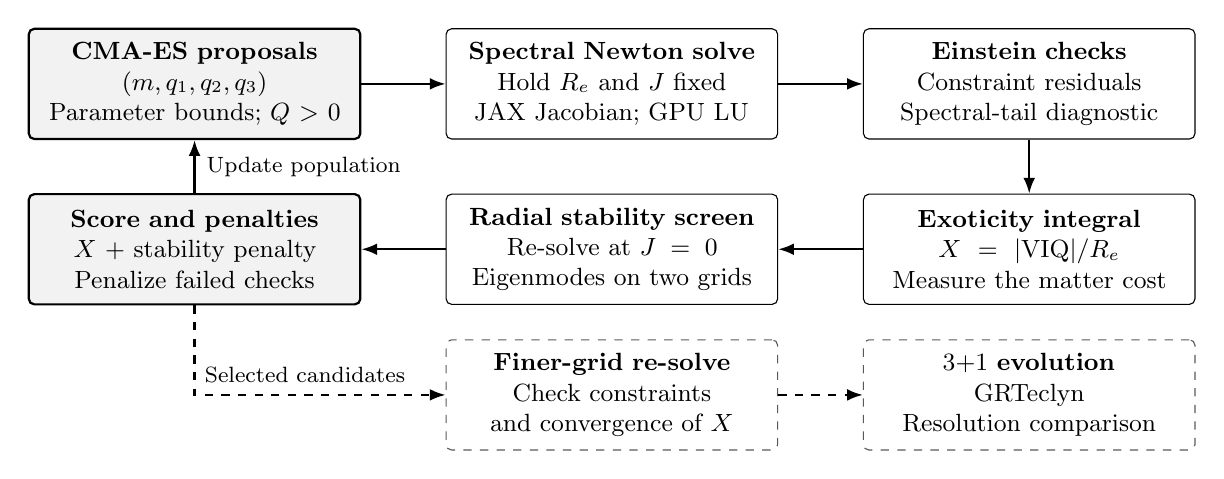
\begin{tikzpicture}[
  font=\small,
  stagebox/.style={draw, rounded corners=2pt, align=center,
    text width=40mm, minimum height=14mm, inner sep=3pt},
  search/.style={stagebox, fill=black!5, thick},
  followup/.style={stagebox, dashed, draw=black!65},
  flow/.style={-{Latex[length=2mm]}, thick},
  note/.style={font=\footnotesize, align=center, fill=white, inner sep=2pt}
]
\node[search] (cma) at (0,0)
  {\textbf{CMA-ES proposals}\\$(m,q_1,q_2,q_3)$\\Parameter bounds; $Q>0$};
\node[stagebox] (newton) at (5.3,0)
  {\textbf{Spectral Newton solve}\\Hold $R_e$ and $J$ fixed\\JAX Jacobian; GPU LU};
\node[stagebox] (constraints) at (10.6,0)
  {\textbf{Einstein checks}\\Constraint residuals\\Spectral-tail diagnostic};
\node[stagebox] (exoticity) at (10.6,-2.1)
  {\textbf{Exoticity integral}\\$X=|\mathrm{VIQ}|/R_e$\\Measure the matter cost};
\node[stagebox] (stability) at (5.3,-2.1)
  {\textbf{Radial stability screen}\\Re-solve at $J=0$\\Eigenmodes on two grids};
\node[search] (score) at (0,-2.1)
  {\textbf{Score and penalties}\\$X$ + stability penalty\\Penalize failed checks};
\draw[flow] (cma)--(newton);
\draw[flow] (newton)--(constraints);
\draw[flow] (constraints)--(exoticity);
\draw[flow] (exoticity)--(stability);
\draw[flow] (stability)--(score);
\draw[flow] (score.north)--node[note, midway, right=2pt] {Update population} (cma.south);
\node[followup] (grid) at (5.3,-3.95)
  {\textbf{Finer-grid re-solve}\\Check constraints\\and convergence of $X$};
\node[followup] (evolve) at (10.6,-3.95)
  {\textbf{$3{+}1$ evolution}\\GRTeclyn\\Resolution comparison};
\draw[flow, dashed] (score.south) |- node[note, pos=0.72, above=2pt]
  {Selected candidates} (grid.west);
\draw[flow, dashed] (grid)--(evolve);
\end{tikzpicture}}
\caption{Optimization of the confining potential at fixed throat size and angular momentum. Each CMA-ES proposal starts Newton iteration from a nearby solved candidate; JAX supplies the Jacobian for the GPU solve. Exoticity, the radial screen and constraint penalties feed back into the search; inadmissible or failed solves receive a penalty. Dashed arrows lead to separate resolution and evolution tests. The loop ranks candidates; the subsequent tests assess their reliability.}
\label{fig:search}
\end{figure*}

\subsection{Spectral Newton solver}
\label{sec:opt:solver}

The compactified coordinate $x=(2/\pi)\arctan(\eta/\eta_0)$ maps both asymptotic ends to $x=\pm1$. The five fields are expanded in Chebyshev polynomials of $x$ and even cosine modes of $\theta$ on a tensor-product Lobatto grid. Damped Newton iteration solves the five coupled elliptic equations for $f$, $\omega$, $N=\nu/\sin^2\theta$, $B$, and $\psi$, bordered by the vacuum value $\psi_-$, a radial length scale $\sigma$, and two constraint rows that pin $J$ and $R_e$, until the residual reaches machine round-off. Here $N$ is the axis-regularized combination introduced to remove the coordinate degeneracy of the $\nu$ equation on the symmetry axis. The dense Jacobian is computed exactly via forward-mode automatic differentiation in \texttt{JAX}~\cite{jax2018} in column blocks and factored on the GPU via dense LU decomposition. Every converged solution is checked against two first-order Einstein constraint identities that never enter the Newton iteration, as well as the spectral decay of the trailing Chebyshev coefficients. At $\mathcal{V}=0$, the solver reproduces the published solutions of Ref.~\cite{shirokov2026s} to machine precision (Appendix~\ref{app:checks}).

\subsection{CMA-ES}
\label{sec:opt:cma}

The outer optimization uses CMA-ES~\cite{hansen01} over the four potential parameters $(m,q_1,q_2,q_3)$. Each evaluation performs a Newton solve, initialized from the nearest previously solved potential in parameter space. Proposals with $Q\le0$, failed Newton solves, or background-constraint residuals above $10^{-6}$ receive a large penalty. Candidates between $10^{-8}$ and $10^{-6}$ receive an additional constraint penalty. The objective also includes a radial perturbation screen of the static counterpart at the same pinned $R_e$. The stationary results reported below are selected by their exoticity and background constraints. A separate finer-grid re-solve supplies the selected D21 solution used for evolution. Figure~\ref{fig:cma} shows its family's recorded search history.

\begin{figure}[!t]
\centering
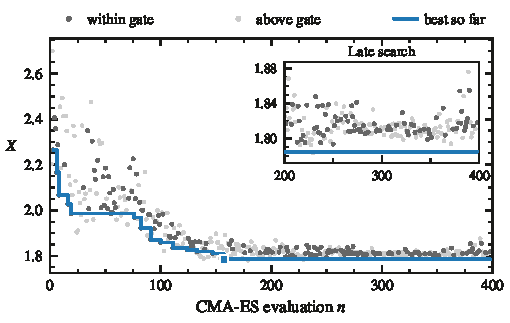
\includegraphics[width=\columnwidth]{cma_progress_d21.pdf}
\caption{Search-grid exoticity $X$ against CMA-ES evaluation for D21. Dark and light grey points lie within and above the background-constraint threshold, respectively. The blue step tracks the running minimum; the square marks its first attainment. The inset resolves the late-search plateau. The search minimum is $X=\clmDsearchX$, whereas the separately selected, finer-grid solution has $X=\clmDfineX$ (Table~\ref{tab:X}).}
\label{fig:cma}
\end{figure}

Figure~\ref{fig:search-regions} shows the sampled parameter regions and search histories for both families. Labels D and S denote drainhole and symmetric searches; the suffix gives the nominal equatorial rotation $100v_e$. The projections combine searches at different fixed angular momenta; overlapping points can differ in the two hidden potential parameters. Each history is normalized to its own first candidate satisfying the background-constraint threshold, so the curves compare progress within a search.

\begin{figure*}[t]
\centering
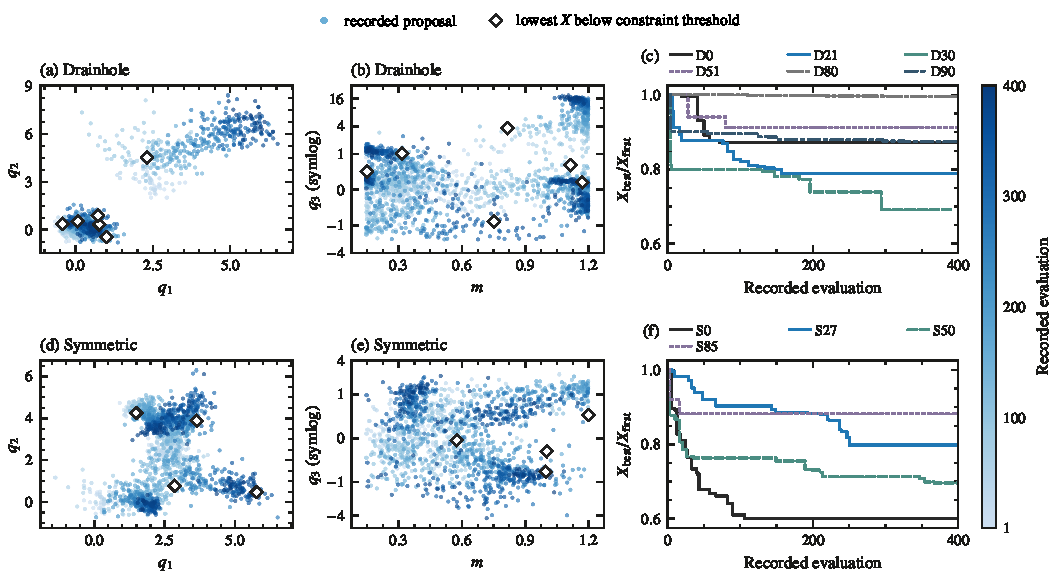
\includegraphics[width=\textwidth]{potential_scans.pdf}
\caption{CMA-ES exploration of the four potential parameters at fixed $R_e$ and $J$, for the drainhole (top) and symmetric (bottom) families. Panels (a,b,d,e) project recorded proposals, coloured by evaluation order; diamonds mark each search's lowest $X$ with both background-constraint residuals below $10^{-6}$. The $q_3$ axes are symmetric-logarithmic, linear for $|q_3|\le1$. Panels (c,f) show the running minimum relative to the first candidate below that threshold. The searches concentrate in distinct parameter regions and approach plateaus at different rates.}
\label{fig:search-regions}
\end{figure*}

\section{Numerical setup}
\label{sec:setup}

\subsection{Interpolation onto the grid}
\label{sec:setup:id}

To evolve the optimized solutions in $3{+}1$ dimensions, the stationary metric~\eqref{eq:metric} is exported as an extended seven-column background table (adding $B$ and the polynomial coefficients of $\mathcal{V}(\psi)$ in the header) and interpolated via $C^2$ cubic splines onto the Cartesian AMR grid through the isotropic radius $r$, where $\eta=r-\eta_0^2/4r$ as in Ref.~\cite{shirokov2026s}. The $\eta\to-\infty$ asymptotic end compactifies to a puncture at $r=0$. The conformal factor incorporates $B$ via $\chi\to\chi/B^2$, while the lapse $\alpha$, shift $\beta^i$, and scalar field $\psi$ are read directly from the table. The extrinsic curvature $K_{ij}$ follows analytically from the stationary shift, and the scalar's initial conjugate momentum vanishes in the corotating frame.

\subsection{Evolution scheme}
\label{sec:setup:scheme}

Nonlinear $3{+}1$ evolutions are performed with \texttt{GRTeclyn}~\cite{grteclyn,amrex,grchombo} using the evolution formulation of Refs.~\cite{shirokov2026,shirokov2026s}: the conformal and covariant Z4 (CCZ4) formulation~\cite{alic2012}, $1{+}\log$ slicing~\cite{bona1995}, Gamma-driver shift~\cite{alcubierre2003gauge}, fourth-order spatial finite differences, fourth-order Runge--Kutta time integration with Courant factor $\Delta t=0.02\,\Delta x$, and Kreiss--Oliger dissipation. The exotic scalar module evaluates the polynomial potential $\mathcal{V}(\psi)$ and its derivative $\mathcal{V}'(\psi)$ directly in the matter evolution kernels and in the Hamiltonian constraint diagnostic. Three nested AMR refinement levels are centered on the throat. The outer sponge driving is disabled in these evolutions.

\subsection{Criteria}
\label{sec:setup:criteria}

The search and validation stages use separate criteria. A search-grid candidate enters Tables~\ref{tab:models} and \ref{tab:X} when both independent background-constraint residuals are at most $10^{-8}$. Each table selects the lowest recorded $X$ satisfying that threshold in the specified search. A selected candidate is then re-solved on a finer grid and checked again. Perturbative stability additionally requires converged eigenvalues and small residuals in the linearized Einstein equations not used by the eigenproblem. A small background residual or exoticity value alone does not establish stability.

\section{Results}
\label{sec:results}

\begin{table*}[t]
\begin{minipage}[t]{0.48\textwidth}
\begin{minipage}[t][64pt][t]{\linewidth}
\caption{Potential parameters of the lowest-$X$ candidates with both background-constraint residuals at most $10^{-8}$ on the $150\times30$ search grid. D and S denote the drainhole and symmetric families. D21$^\star$ is the separately selected solution re-solved on $210\times42$, rather than the search-grid minimum.}
\label{tab:models}
\end{minipage}\par
\scriptsize
\begin{ruledtabular}
\begin{tabular}{lrrrr}
model & $m$ & $q_1$ & $q_2$ & $q_3$ \\
\hline
\clmModelsRows
\end{tabular}
\end{ruledtabular}
\end{minipage}\hfill
\begin{minipage}[t]{0.48\textwidth}
\begin{minipage}[t][64pt][t]{\linewidth}
\caption{Exoticity of the same candidates as Table~\ref{tab:models}, compared with the massless solution at the same $R_e$ and $J$. Here $\Delta X=100(X/X_{\mathcal{V}=0}-1)$. The search-grid rows and the selected finer-grid solution are listed separately.}
\label{tab:X}
\end{minipage}\par
\scriptsize
\begin{ruledtabular}
\begin{tabular}{lrrr}
model & $X$ & $X_{\mathcal{V}=0}$ & $\Delta X$ \\
\hline
\clmExoticityRows
\end{tabular}
\end{ruledtabular}
\end{minipage}
\end{table*}

\subsection{\texorpdfstring{Stationary exoticity at fixed throat and spin}{Stationary exoticity at fixed throat and spin}}
\label{sec:results:X}

The fixed-$R_e$, fixed-$J$ searches cover both static and rotating members of the drainhole and symmetric families. Tables~\ref{tab:models} and \ref{tab:X} use the same candidate selection and list the two families separately. Their search-grid rows characterize the numerical optimization at that resolution. Figure~\ref{fig:exotic} compares these candidates with the classical massless families.

\begin{figure}[!t]
\centering
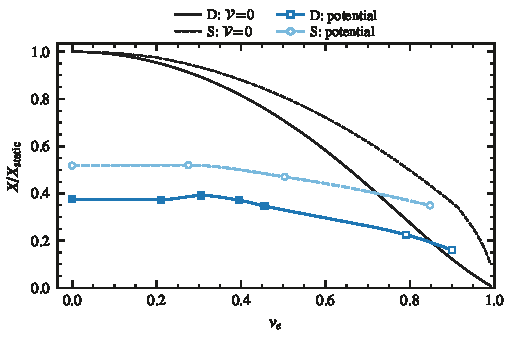
\includegraphics[width=\columnwidth]{exotic_spin.pdf}
\caption{Exoticity relative to each family's massless static member, against the reference rotation $v_e$. Black curves: massless families. Open blue markers: the search-grid candidates of Table~\ref{tab:X}. The filled diamond identifies D21$^\star$ on $210\times42$. Most search candidates lie below their massless counterparts; D90 lies above its counterpart.}
\label{fig:exotic}
\end{figure}

The search-grid candidates reduce $X$ at most sampled rotations, but the high-spin D90 candidate has a larger exoticity than the corresponding massless solution. The optimized coefficients also include negative values of individual $q_i$; admissibility requires positivity of the full polynomial $Q(u)$ between the vacua. A positive value of every coefficient is not required.

The separately selected D21$^\star$ solution has $X=\clmDfineX$ on $210\times42$, a reduction of $\clmDfineReduction\%$ at fixed throat radius and angular momentum. Its independent background-constraint residuals are $E_{19}=\clmDfineEoneNine$ and $E_c=\clmDfineEc$. This solution supplies the initial data for the three-dimensional resolution study.

\subsection{\texorpdfstring{Three-dimensional evolution of D21$^\star$}{Three-dimensional evolution of D21*}}
\label{sec:results:evol}

We evolved D21$^\star$ at base resolutions $N=96,128,192$ with the same domain and refinement hierarchy. During the common early-time interval, the near-throat constraint norms exhibit approximately fourth-order scaling. The other refinement levels show more variable orders (Appendix~\ref{app:conv}).

The throat subsequently contracts at all three resolutions. Its equatorial radius first falls by one percent at $t=\clmContractionLow$, $\clmContractionMid$, and $\clmContractionHigh$, respectively. The onset moves later as the grid is refined. Figure~\ref{fig:conv} shows this resolution dependence directly, together with the areal-radius, wave-extraction, and lapse diagnostics. The early constraint scaling supports the discretization check; the delayed contraction is a separate feature of the evolution.

\section{Conclusions}
\label{sec:conclusions}

A spectral Newton solver coupled to CMA-ES identifies confining phantom potentials with lower stationary exoticity at fixed throat size and angular momentum. Independent Einstein constraints provide an essential check on each candidate. The search-grid tables summarize the explored families, while the selected finer-grid D21$^\star$ solution retains a $\clmDfineReductionRounded\%$ reduction relative to the massless phantom. The benefit depends on the reference rotation: the D90 search candidate has a larger matter cost than its massless counterpart. The three-dimensional D21$^\star$ evolutions show early constraint convergence and later contraction whose onset shifts with resolution. These measurements distinguish a reduction in stationary matter content from a conclusion about dynamical stability.

\section{Reproducibility}
\label{sec:data}

The solver, optimization and figure-generation scripts are available in the \texttt{GRTeclyn} research repository~\cite{shirokov2026code}. The archived search traces identify every candidate used in Tables~\ref{tab:models} and \ref{tab:X}; a checked selection ledger generates both tables. The selected D21$^\star$ field arrays and the final evolution diagnostic streams are included with the figure inputs. All article figures rebuild from those tracked data.

\begin{figure*}[t]
\centering
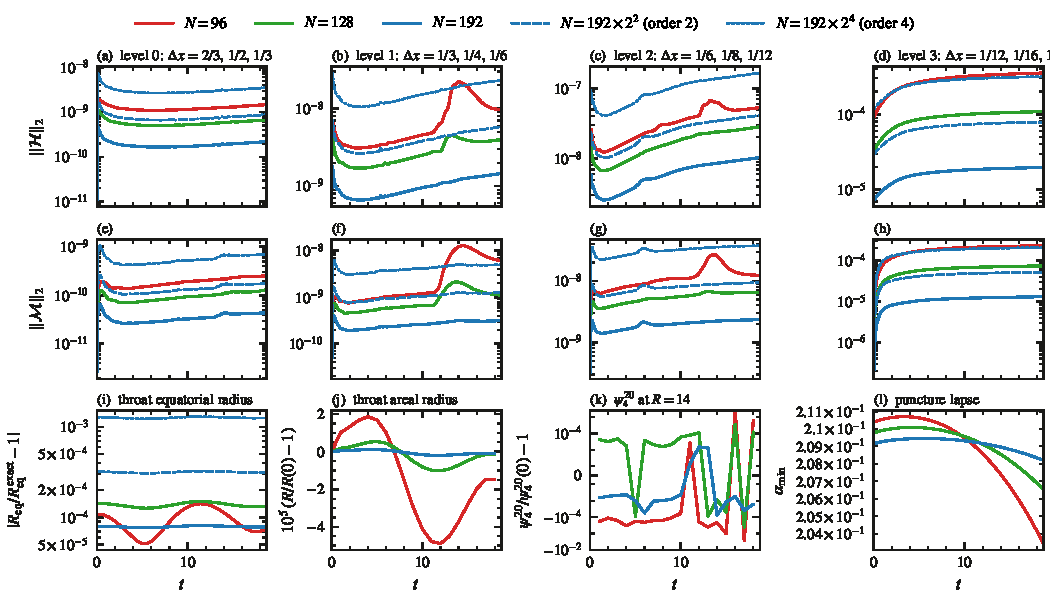
\includegraphics[width=\textwidth]{convergence_d21.pdf}
\caption{Resolution study of D21$^\star$ at $N=96,128,192$. Top two rows: Hamiltonian and momentum constraint norms through $t=50$; grey dashed and dotted curves multiply the finest-grid norms by $2^2$ and $2^4$. Bottom row: fractional equatorial- and areal-radius changes, the change in $r\,\mathrm{Re}\,\Psi_4^{20}$ at $r=14$, and minimum lapse over each recorded history. Near-throat constraints scale approximately at fourth order early on; the later contraction begins at resolution-dependent times.}
\label{fig:conv}
\end{figure*}

\begin{acknowledgments}
This work was supported by Gravity Frontiers
(\url{https://www.gravityfrontiers.org/en}), which funded the underlying
research and the development of the numerical-simulation software. The authors
acknowledge the GRTL Collaboration for \texttt{GRChombo}, \texttt{GRTresna},
and \texttt{GRTeclyn}.
\end{acknowledgments}

\appendix

\section{Solver and stability checks}
\label{app:checks}

At $\mathcal{V}=0$, the five-field spectral residual reduces symbolically to the published spinning wormhole system of Ref.~\cite{shirokov2026s}, and Newton iteration across the saved solutions of that work reproduces their global charges, $B\equiv 1$, and Fig.~3e exoticity values $X$ to machine precision. During the $\mathcal{V}\neq 0$ search, the two first-order Einstein equations omitted from the five-equation elliptic solve---the $\eta\theta$ Einstein component and the pointwise generalization of the $D^2$ conservation identity of Ref.~\cite{chew2016}---serve as independent monitors. The search-grid selection and the separate finer-grid check both use these monitors, as described in Sec.~\ref{sec:setup:criteria}.

The linear radial stability screen computes the spherical ($m=0$) perturbation spectrum of the $J=0$ background at the candidate's pinned throat radius $R_e$ in a regular conformal chart. Linearizing the Einstein--Klein--Gordon system yields three coupled radial wave equations cast as a dense generalized eigenvalue problem on Chebyshev--Lobatto grids. Because continuous gauge modes survive discretization at the boundaries, a physical mode must satisfy both two-grid eigenvalue convergence and the independent linearized Einstein constraints ($tt$ and $t\eta$). On the classical $\mathcal{V}=0$ backgrounds, this pipeline reproduces the published growth rates $|\omega_I|\eta_0=0.390$ for the static drainhole~\cite{azad2023,azad2024} and $|\omega_I|\eta_0=1.182$ for the symmetric Ellis throat. The stationary tables are selected using the background equations. Stability is an additional property of the perturbation spectrum and its independent constraints.

\section{Convergence of the D21 evolution}
\label{app:conv}

D21$^\star$ was evolved at base resolutions $N=96,128,192$ on a domain of length $L=64$ with three additional refinement levels. Figure~\ref{fig:conv} uses the final recorded diagnostic streams. The top two rows compare constraints at equal times through $t=50$; the bottom row follows each simulation to its final diagnostic sample. The areal-radius diagnostic uses the minimum area of coordinate spheres, and the wave diagnostic is the change in $r\,\mathrm{Re}\,\Psi_4^{20}$ at extraction radius $r=14$.

Because the exact constraint values vanish, their norms can be compared directly under refinement. The measured pairwise order is
\begin{equation}
p_{a\to b}(t)=\frac{\ln[C_{N_a}(t)/C_{N_b}(t)]}{\ln(N_b/N_a)},
\label{eq:order}
\end{equation}
where $C_N$ is a constraint norm on the same refinement level. Table~\ref{tab:orders} gives both neighboring-resolution comparisons. The finest level is close to fourth order over the reported interval, whereas intermediate levels exhibit mixed orders and transients. The throat-radius histories later separate in time as contraction develops; that behavior is not described by a uniform convergence order for the full evolution.

\begin{table*}[t]
\caption{Measured constraint orders from Eq.~\eqref{eq:order}. Each cell gives $96\to128$ / $128\to192$ at the same time and refinement level. Norms are linearly interpolated between recorded times. The finest-level orders stay near four; the coarser levels vary with time and resolution pair.}
\label{tab:orders}
\small
\begin{ruledtabular}
\begin{tabular}{lccccc}
constraint & $t=10$ & $t=20$ & $t=30$ & $t=40$ & $t=50$ \\
\hline
\clmOrderRows
\end{tabular}
\end{ruledtabular}
\end{table*}


\begin{thebibliography}{99}

\bibitem{ellis1973}
H.~G.~Ellis,
\newblock ``Ether flow through a drainhole: A particle model in general relativity,''
\newblock J.\ Math.\ Phys.\ \textbf{14}, 104 (1973).

\bibitem{bronnikov1973}
K.~A.~Bronnikov,
\newblock ``Scalar-tensor theory and scalar charge,''
\newblock Acta Phys.\ Polon.\ B \textbf{4}, 251 (1973).

\bibitem{morris_thorne1988}
M.~S.~Morris and K.~S.~Thorne,
\newblock ``Wormholes in spacetime and their use for interstellar travel: A tool for teaching general relativity,''
\newblock Am.\ J.\ Phys.\ \textbf{56}, 395 (1988).

\bibitem{visser1995}
M.~Visser,
\newblock \emph{Lorentzian Wormholes: From Einstein to Hawking}
\newblock (AIP Press, Woodbury, NY, 1995).

\bibitem{gonzalez2009lin}
J.~A.~Gonz\'alez, F.~S.~Guzm\'an, and O.~Sarbach,
\newblock ``Instability of wormholes supported by a ghost scalar field. I. Linear stability analysis,''
\newblock Class.\ Quantum Grav.\ \textbf{26}, 015010 (2009).

\bibitem{gonzalez2009}
J.~A.~Gonz\'alez, F.~S.~Guzm\'an, and O.~Sarbach,
\newblock ``Instability of wormholes supported by a ghost scalar field. II. Nonlinear evolution,''
\newblock Class.\ Quantum Grav.\ \textbf{26}, 015011 (2009).

\bibitem{visser2003}
M.~Visser, S.~Kar, and N.~Dadhich,
\newblock ``Traversable wormholes with arbitrarily small energy condition violations,''
\newblock Phys.\ Rev.\ Lett.\ \textbf{90}, 201102 (2003).

\bibitem{fewster2005}
C.~J.~Fewster and T.~A.~Roman,
\newblock ``On wormholes with arbitrarily small quantities of exotic matter,''
\newblock Phys.\ Rev.\ D \textbf{72}, 044023 (2005).

\bibitem{kuhfittig2008}
P.~K.~F.~Kuhfittig,
\newblock ``Viable models of traversable wormholes supported by small amounts of exotic matter,''
\newblock arXiv:0806.1194 [gr-qc] (2008).

\bibitem{dzhunushaliev2014topology}
V.~Dzhunushaliev, V.~Folomeev, C.~Hoffmann, B.~Kleihaus, and J.~Kunz,
\newblock ``Boson Stars with Nontrivial Topology,
\newblock Phys.\ Rev.\ D \textbf{90}, 124038 (2014),
\newblock \href{https://arxiv.org/abs/1409.6978}{arXiv:1409.6978 [gr-qc]}.

\bibitem{kleihaus_kunz2014}
B.~Kleihaus and J.~Kunz,
\newblock ``Rotating Ellis wormholes in four dimensions,''
\newblock Phys.\ Rev.\ D \textbf{90}, 121503(R) (2014).

\bibitem{chew2016}
X.~Y.~Chew, B.~Kleihaus, and J.~Kunz,
\newblock ``Geometry of spinning Ellis wormholes,''
\newblock Phys.\ Rev.\ D \textbf{94}, 104031 (2016).

\bibitem{azad2023}
B.~Azad, J.~L.~Bl\'azquez-Salcedo, F.~S.~Khoo, and J.~Kunz,
\newblock ``Are slowly rotating Ellis--Bronnikov wormholes stable?,''
\newblock Phys.\ Lett.\ B \textbf{848}, 138349 (2024).

\bibitem{azad2024}
B.~Azad, J.~L.~Bl\'azquez-Salcedo, F.~S.~Khoo, and J.~Kunz,
\newblock ``Radial perturbations of Ellis--Bronnikov wormholes in slow rotation up to second order,''
\newblock Phys.\ Rev.\ D \textbf{109}, 124051 (2024).

\bibitem{shirokov2026}
N.~M.~Shirokov,
\newblock ``Wormhole dynamics: nonlinear collapse and gravitational-wave emission,''
\newblock arXiv:2604.00071 [gr-qc] (2026).

\bibitem{shirokov2026s}
N.~M.~Shirokov and I.~Nachevsky,
\newblock ``Rotation slows the instability of Ellis--Bronnikov wormholes,''
\newblock arXiv:2610.29941 [gr-qc] (2026).

\bibitem{helmerich2024warpfactory}
C.~Helmerich, J.~Fuchs, A.~Bobrick, L.~Sellers, B.~Melcher, and G.~Martire,
\newblock ``Analyzing warp drive spacetimes with Warp Factory,''
\newblock Class.\ Quantum Grav.\ \textbf{41}, 095009 (2024).

\bibitem{hansen01}
N.~Hansen and A.~Ostermeier,
\newblock ``Completely derandomized self-adaptation in evolution strategies,''
\newblock Evol.\ Comput.\ \textbf{9}, 159 (2001).

\bibitem{jax2018}
J.~Bradbury, R.~Frostig, P.~Hawkins, M.~J.~Johnson, C.~Leary, D.~Maclaurin, G.~Necula, A.~Paszke, J.~VanderPlas, S.~Wanderman-Milne, and Q.~Zhang,
\newblock \texttt{JAX}: composable transformations of Python+NumPy programs,
\newblock \url{https://github.com/jax-ml/jax} (2018).

\bibitem{alic2012}
D.~Alic, C.~Bona-Casas, C.~Bona, L.~Rezzolla, and C.~Palenzuela,
\newblock ``Conformal and covariant formulation of the Z4 system with constraint-violation damping,''
\newblock Phys.\ Rev.\ D \textbf{85}, 064040 (2012).

\bibitem{bona1995}
C.~Bona, J.~Mass\'o, E.~Seidel, and J.~Stela,
\newblock ``New formalism for numerical relativity,''
\newblock Phys.\ Rev.\ Lett.\ \textbf{75}, 600 (1995).

\bibitem{alcubierre2003gauge}
M.~Alcubierre, B.~Br\"ugmann, P.~Diener, M.~Koppitz, D.~Pollney, E.~Seidel, and T.~Takahashi,
\newblock ``Gauge conditions for long-term numerical black hole evolutions without excision,''
\newblock Phys.\ Rev.\ D \textbf{67}, 084023 (2003).

\bibitem{grteclyn}
GRTL Collaboration,
\newblock \texttt{GRTeclyn},
\newblock \url{https://github.com/GRTLCollaboration/GRTeclyn}.

\bibitem{amrex}
W.~Zhang \emph{et al.},
\newblock ``AMReX: a framework for block-structured adaptive mesh refinement,''
\newblock J.\ Open Source Softw.\ \textbf{4}, 1370 (2019).

\bibitem{grchombo}
T.~Andrade \emph{et al.},
\newblock ``GRChombo: an adaptable numerical relativity code for fundamental physics,''
\newblock J.\ Open Source Softw.\ \textbf{6}, 3703 (2021).

\bibitem{shirokov2026code}
N.~M.~Shirokov and I.~Nachevsky,
\newblock \texttt{GRTeclyn} research fork,
\newblock \url{https://github.com/Nikchik-coder/GRTeclyn},
\newblock doi:\href{https://doi.org/10.5281/zenodo.23245933}{10.5281/zenodo.23245933} (2026).

\end{thebibliography}

\end{document}
